% !TEX root = ../main.tex
% ---------------------------------------------------------------
% GOALS
% ---------------------------------------------------------------



\chapter{Motivazioni ed obiettivi}\label{chap4:Goals}

\begin{tikzpicture}
\node [mybox] (box){%
	\begin{minipage}{.96\textwidth}
	Quello che, dunque, si vuole dimostrare è innanzitutto l'esistenza di una nuova classe chiamata preFoG e che sia divisa da quelle di FoG e noFoG. Una volta dimostrato questo, si vuole trovare il miglior intervallo di suddivisione dei dati al fine di sviluppare un procedimento di riconoscimento non supervisionato di etichette delle varie classi attraverso algoritmi di clustering, sostituendo cosí il dottore nella prima fase di test. Sfruttando tale intervallo, inoltre, si vuole tentare un primo approccio di classificazione per poter etichettare nuovi dati rispetto a quelli contenuti nel nostro dataset di allenamento.
	\end{minipage}
};
\end{tikzpicture}%

\begin{figure}[]
	\centering
	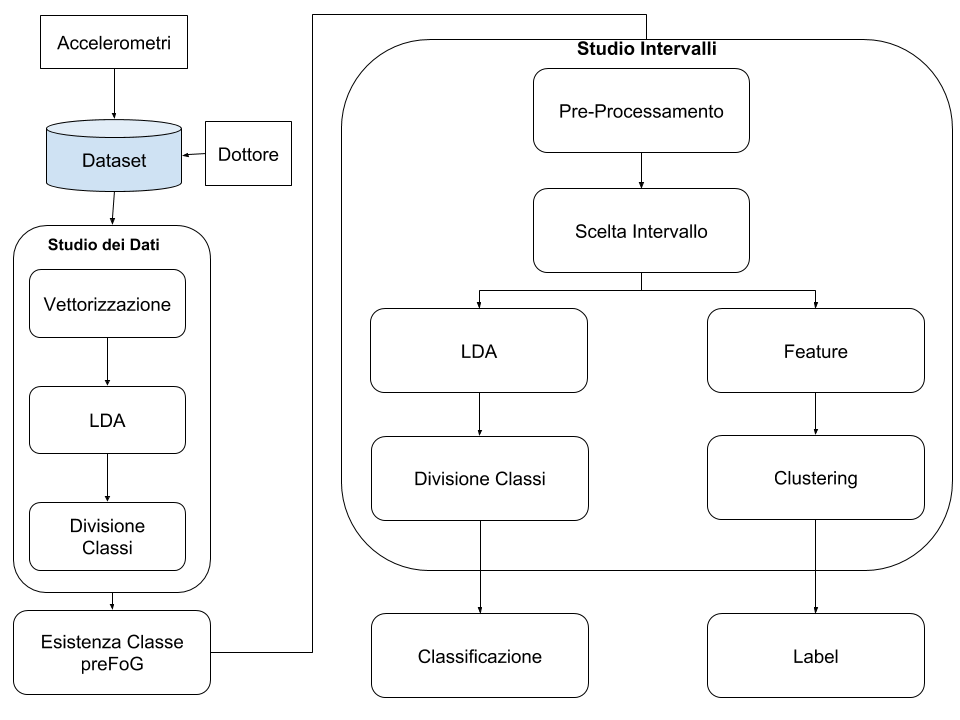
\includegraphics[scale=0.35]{images/FlussoTesi.png}
	\caption{Rappresentazione del flusso della tesi}
	\label{FlussoTesi1}
\end{figure}
